\section{Casi d'uso}
In seguito ad un'analisi approfondita del capitolato, ad un incontro con il proponente \Zucchetti\ e ad una discussione tra gli Analisti, sono emersi i seguenti casi d'uso.\\
Ogni caso d'uso è identificato da un codice univoco che ne rappresenta anche la posizione all'interno della gerarchia; il codice è così composto:
\begin{center}
UC[codice rappresentante il padre].[codice progressivo]
\end{center}
Il codice progressivo può avanzare nei livelli di gerarchia divindendo tali livelli con un punto.
\newpage
\subsection{Gerarchia degli utenti}
La seguente gerarchia di utenti viene considerata valida in tutti i casi d'uso:
\begin{figure}[h]
\begin{center}
	 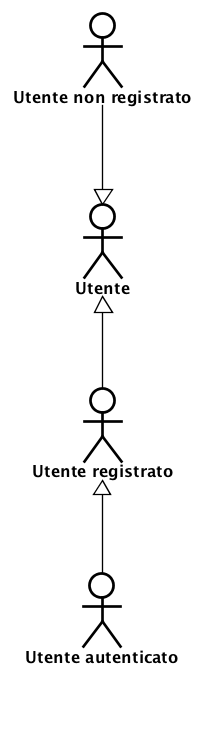
\includegraphics[scale=0.5]{diagram/gerarchia.png}
\end{center}
\end{figure}
\newpage

\subsection{ UC0: Premi}
\begin{figure}[h]
	\begin{center}
	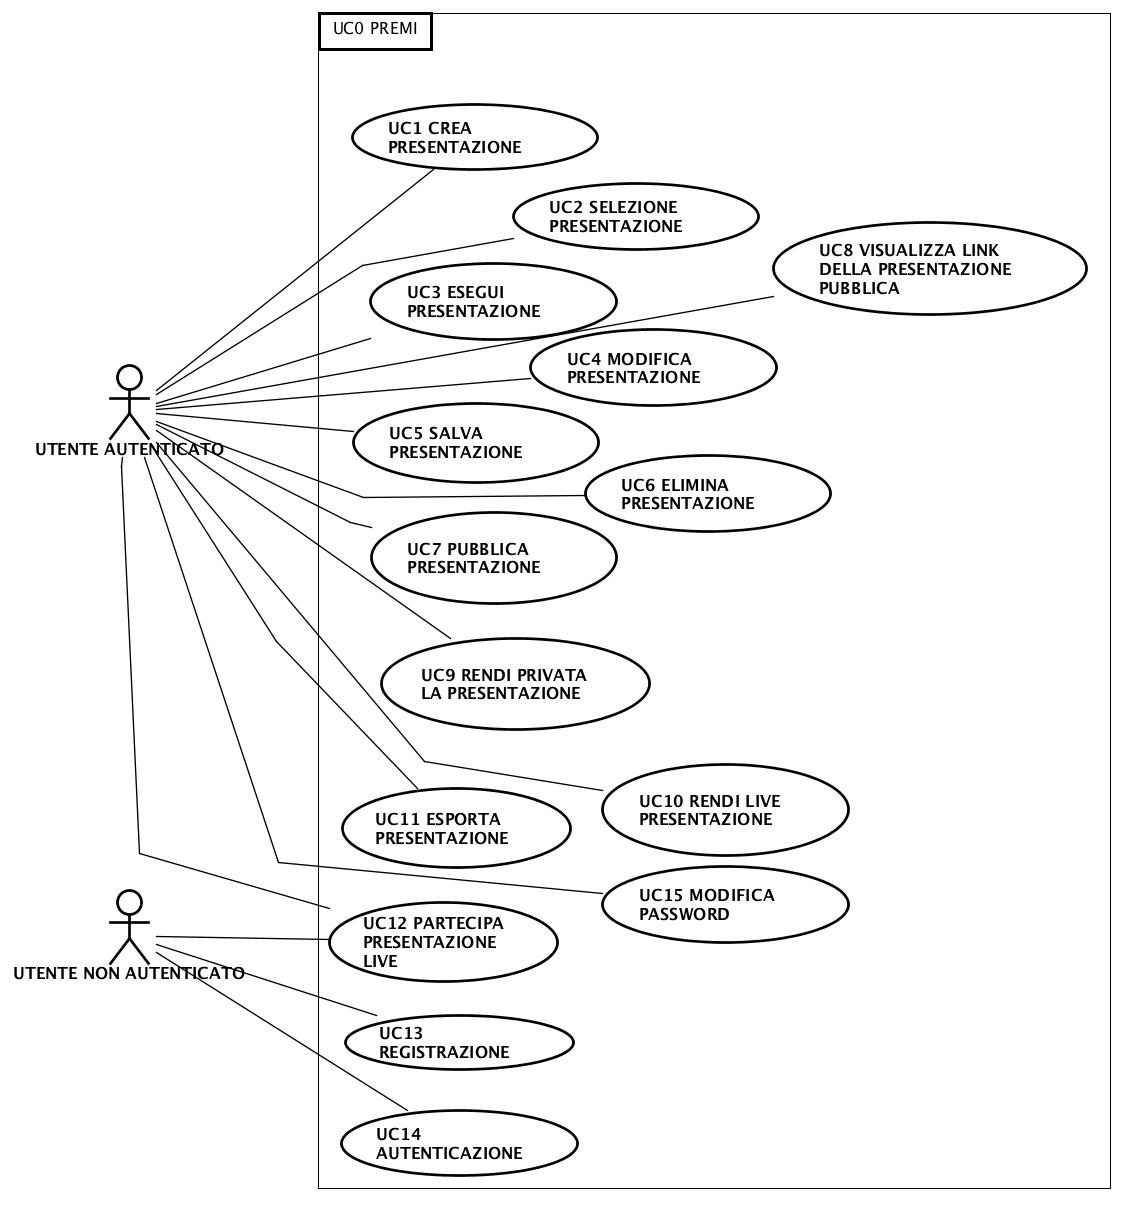
\includegraphics[scale=0.4]{diagram/UC0.png}
	\caption{Caso d'uso UC0}
	\end{center}
\end{figure}
\begin{itemize}
	\item \textbf{Precondizione:} Il sistema è avviato;
	\item \textbf{Postcondizione:} Il sistema ha eseguito le operazioni che l'utente ha richiesto;
	\item \textbf{Descrizione:} L'utente accede alle funzionalità del sistema;
	\item \textbf{Attori:} Utente non registrato, Utente, Utente registrato, Utente autenticato;
	\item \textbf{Scenario principale:}
	\begin{enumerate}
		\item \textbf{ UC1:} \textit{ Registrazione};
		\item \textbf{ UC2:} \textit{ Notifiche di sistema};
		\item \textbf{ UC3:} \textit{ Partecipazione presentazione live};
		\item \textbf{ UC4:} \textit{ Autenticazione};
		\item \textbf{ UC5:} \textit{ Elenco presentazioni};
		\item \textbf{ UC6:} \textit{ Modifica dati account};
		\item \textbf{ UC7:} \textit{ Nuova presentazione};
		\item \textbf{ UC8:} \textit{ Selezione template$_G$};
		\item \textbf{ UC9:} \textit{ Visualizza presentazione condivisa}.
	\end{enumerate}
\end{itemize}
\newpage
\subsection{ UC1: Registrazione}

\begin{figure}[h]
	\begin{center}
	\includegraphics[scale=0.4]{diagram/UC1.png}
	\caption{Caso d'uso UC1}
	\end{center}
\end{figure}
\begin{itemize}
	\item \textbf{Precondizione:} L'utente ha scelto di registrarsi;
	\item \textbf{Postcondizione:} L'utente verrà registrato nel database$_G$;
	\item \textbf{Descrizione:} L'utente può registrarsi al sistema;
	\item \textbf{Attori:} Utente non registrato;
	\item \textbf{Scenario principale:}
	\begin{enumerate}
		\item \textbf{ UC1.1:} \textit{ Inserimento username};
		\item \textbf{ UC1.2:} \textit{ Inserimento password};
		\item \textbf{ UC1.3:} \textit{ Inserimento conferma password};
		\item \textbf{ UC1.4:} \textit{ Inserimento e-mail};
		\item \textbf{ UC1.5:} \textit{ Conferma registrazione};
		\item \textbf{ UC1.6:} \textit{ Annulla registrazione}.
	\end{enumerate}
\end{itemize}
\subsection{ UC1.1: Inserimento username}

\begin{itemize}
	\item \textbf{Precondizione:} L'utente ha scelto di registrarsi;
	\item \textbf{Postcondizione:} Verrà visualizzato lo username scelto;
	\item \textbf{Descrizione:} L'utente può inserire lo username nel apposito spazio;
	\item \textbf{Attori:} Utente non registrato.
\end{itemize}
\subsection{ UC1.2: Inserimento password}

\begin{itemize}
	\item \textbf{Precondizione:} L'utente ha scelto di registrarsi;
	\item \textbf{Postcondizione:} L'utente avrà inserito la password nel apposito spazio;
	\item \textbf{Descrizione:} L'utente inserisce la password;
	\item \textbf{Attori:} Utente non registrato.
\end{itemize}
\subsection{ UC1.3: Inserimento conferma password}

\begin{itemize}
	\item \textbf{Precondizione:} L'utente ha scelto di registrarsi;
	\item \textbf{Postcondizione:} Viene visualizzato l'inserimento della conferma della password;
	\item \textbf{Descrizione:} L'utente inserisce nuovamente la password;
	\item \textbf{Attori:} Utente non registrato.
\end{itemize}
\subsection{ UC1.4: Inserimento e-mail}

\begin{itemize}
	\item \textbf{Precondizione:} L'utente ha scelto di registrarsi;
	\item \textbf{Postcondizione:} Viene visualizzato l'inserimento del e-mail;
	\item \textbf{Descrizione:} L'utente inserisce la sua e-mail;
	\item \textbf{Attori:} Utente non registrato.
\end{itemize}
\subsection{ UC1.5: Conferma registrazione}

\begin{itemize}
	\item \textbf{Precondizione:} Tutti i dati richiesti sono stati inseriti correttamente;
	\item \textbf{Postcondizione:} L'utente verrà registrato nel database$_G$;
	\item \textbf{Descrizione:} L'utente, dopo aver inserito tutti i dati necessari, conferma di volersi registrare;
	\item \textbf{Attori:} Utente non registrato.
\end{itemize}
\subsection{ UC1.6: Annulla registrazione}

\begin{itemize}
	\item \textbf{Precondizione:} L'utente ha scelto di registrarsi;
	\item \textbf{Postcondizione:} La registrazione verrà annullata e il sistema torna allo stato precedente alla registrazione;
	\item \textbf{Descrizione:} L'utente può scegliere di non registrarsi;
	\item \textbf{Attori:} Utente non registrato.
\end{itemize}
\subsection{ UC2: Notifiche di sistema}

\begin{itemize}
	\item \textbf{Precondizione:} Il sistema funziona correttamente sia lato server$_G$ sia lato client$_G$;
	\item \textbf{Postcondizione:} Viene notificata un anomalia o un informazione;
	\item \textbf{Descrizione:} In qualunque momento nell'esecuzione dell'applicazione il sistema fa visualizzare all'utente un messaggio di errore, warning o informativo;
	\item \textbf{Attori:} Utente.
\end{itemize}
\subsection{ UC3: Partecipazione presentazione live}

\begin{itemize}
	\item \textbf{Precondizione:} L'utente possiede la URL$_G$ della presentazione che vuole visualizzare e la presentazione è stata resa live;
	\item \textbf{Postcondizione:} L'utente assiste alla presentazione;
	\item \textbf{Descrizione:} L'utente può visualizzare una presentazione resa live precedentemente da un altro utente;
	\item \textbf{Attori:} Utente.
\end{itemize}
\subsection{ UC4: Autenticazione}

\begin{figure}[h]
	\begin{center}
	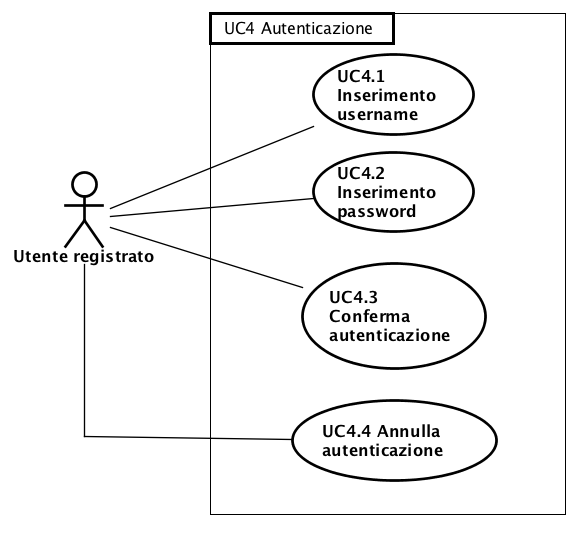
\includegraphics[scale=0.4]{diagram/UC4.png}
	\caption{Caso d'uso UC4}
	\end{center}
\end{figure}
\begin{itemize}
	\item \textbf{Precondizione:} L'utente è registrato e ha scelto di autenticarsi;
	\item \textbf{Postcondizione:} L'utente effettua il login;
	\item \textbf{Descrizione:} Un utente registrato può autenticarsi nel sistema rendendo cosi possibile l'accesso a tutte le funzionalità private di Premi$_G$;
	\item \textbf{Attori:} Utente registrato;
	\item \textbf{Scenario principale:}
	\begin{enumerate}
		\item \textbf{ UC4.1:} \textit{ Inserimento username};
		\item \textbf{ UC4.2:} \textit{ Inserimento password};
		\item \textbf{ UC4.3:} \textit{ Conferma autenticazione};
		\item \textbf{ UC4.4:} \textit{ Annulla autenticazione}.
	\end{enumerate}
\end{itemize}
\subsection{ UC4.1: Inserimento username}

\begin{itemize}
	\item \textbf{Precondizione:} L'utente ha scelto di autenticarsi;
	\item \textbf{Postcondizione:} Viene visualizzato, nel relativo spazio, lo username scritto dall'utente;
	\item \textbf{Descrizione:} Dopo aver scelto di autenticarsi l'utente dovrà inserire il proprio username;
	\item \textbf{Attori:} Utente registrato.
\end{itemize}
\subsection{ UC4.2: Inserimento password}

\begin{itemize}
	\item \textbf{Precondizione:} L'utente ha scelto di autenticarsi e ha scelto di inserire la password;
	\item \textbf{Postcondizione:} L'inserimento della password viene visualizzato nel relativo spazio;
	\item \textbf{Descrizione:} L'utente dopo aver scelto di autenticarsi può inserire la password;
	\item \textbf{Attori:} Utente registrato.
\end{itemize}
\subsection{ UC4.3: Conferma autenticazione}

\begin{itemize}
	\item \textbf{Precondizione:} L'utente ha scelto di autenticarsi e ha inserito password e username;
	\item \textbf{Postcondizione:} L'utente si autentica al sistema;
	\item \textbf{Descrizione:} L'utente può confermare l'autenticazione;
	\item \textbf{Attori:} Utente registrato.
\end{itemize}
\subsection{ UC4.4: Annulla autenticazione}

\begin{itemize}
	\item \textbf{Precondizione:} L'utente ha scelto di autenticarsi;
	\item \textbf{Postcondizione:} Il sistema torna allo stato precedente la scelta di autenticarsi;
	\item \textbf{Descrizione:} L'utente può scegliere di annullare l'autenticazione;
	\item \textbf{Attori:} Utente registrato.
\end{itemize}
\subsection{ UC5: Visualizzazione elenco presentazioni}

\begin{figure}[h]
	\begin{center}
	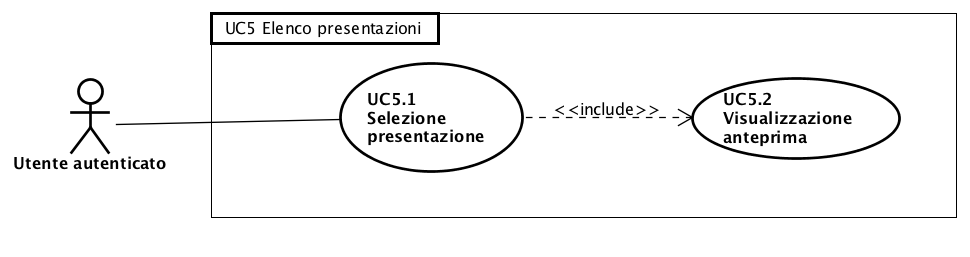
\includegraphics[scale=0.4]{diagram/UC5.png}
	\caption{Caso d'uso UC5}
	\end{center}
\end{figure}
\begin{itemize}
	\item \textbf{Precondizione:} L'utente è nella propria pagina;
	\item \textbf{Postcondizione:} Viene visualizzato l'elenco di tutte le presentazioni dell'utente;
	\item \textbf{Descrizione:} L'utente può scegliere di visualizzare le presentazioni che ha fatto fino a quel momento. Nel caso non ne abbia create l'elenco sarà vuoto;
	\item \textbf{Attori:} Utente autenticato;
	\item \textbf{Scenario principale:}
	\begin{enumerate}
		\item \textbf{ UC5.1:} \textit{ Selezione presentazione};
		\item \textbf{ UC5.2:} \textit{ Visualizzazione anteprima }.
	\end{enumerate}
\end{itemize}

\newpage
\subsection{ UC5.1: Selezione presentazione}

\begin{figure}[h]
	\begin{center}
	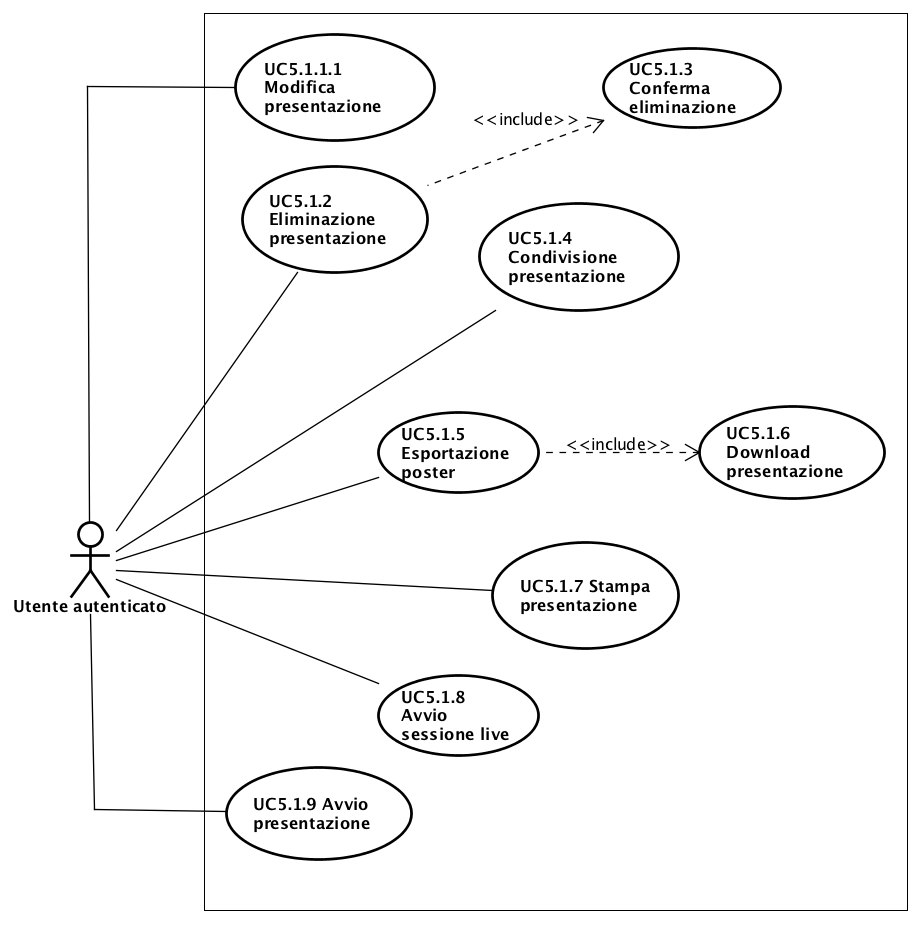
\includegraphics[scale=0.4]{diagram/UC5-1.png}
	\caption{Caso d'uso UC5.1}
	\end{center}
\end{figure}
\begin{itemize}
	\item \textbf{Precondizione:} L'utente ha visualizzato la lista delle sue presentazioni;
	\item \textbf{Postcondizione:} La selezione viene visualizzata insieme all'anteprima della presentazione;
	\item \textbf{Descrizione:} L'utente può selezionare una presentazione accedendo cosi a tutte le sue funzionalità;
	\item \textbf{Attori:} Utente autenticato;
	\item \textbf{Scenario principale:}
	\begin{enumerate}
		\item \textbf{ UC5.1.1:} \textit{ Modifica presentazione};
		\item \textbf{ UC5.1.2:} \textit{ Eliminazione presentazione};
		\item \textbf{ UC5.1.3:} \textit{ Conferma eliminazione};
		\item \textbf{ UC5.1.4:} \textit{ Condivisione presentazione};
		\item \textbf{ UC5.1.5:} \textit{ Esportazione poster};
		\item \textbf{ UC5.1.6:} \textit{ Download presentazione};
		\item \textbf{ UC5.1.7:} \textit{ Stampa presentazione};
		\item \textbf{ UC5.1.8:} \textit{ Avvio sessione live};
		\item \textbf{ UC5.1.9:} \textit{ Avvio presentazione}.
	\end{enumerate}
\end{itemize}
\subsection{ UC5.1.1: Modifica presentazione}

\begin{figure}[h]
	\begin{center}
	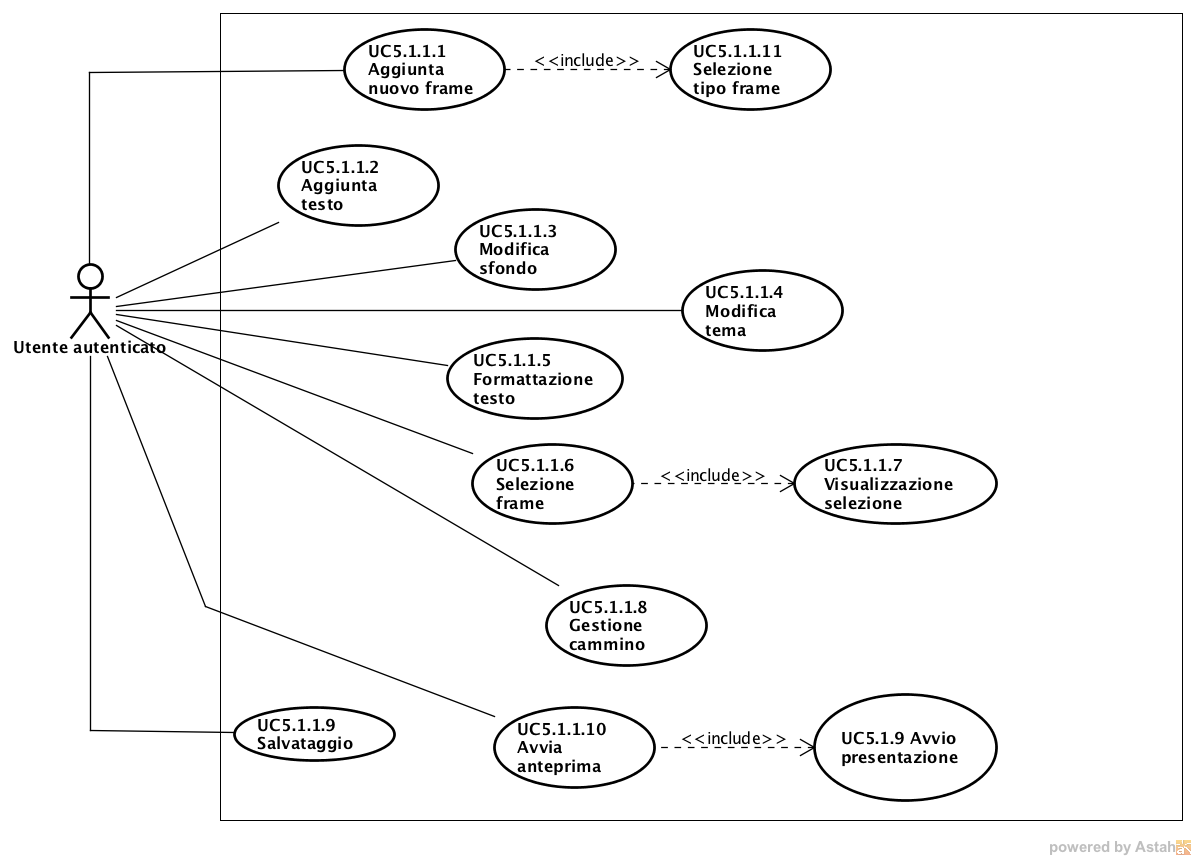
\includegraphics[scale=0.4]{diagram/UC5-1-1.png}
	\caption{Caso d'uso UC5.1.1}
	\end{center}
\end{figure}
\begin{itemize}
	\item \textbf{Precondizione:} L'utente ha selezionato una presentazione;
	\item \textbf{Postcondizione:} Le modifiche apportate dall'utente verranno visualizzate;
	\item \textbf{Descrizione:} L'utente può modificare la presentazione scelta inserendo nuovi oggetti o modificando quelli già esistenti;
	\item \textbf{Attori:} Utente autenticato;
	\item \textbf{Scenario principale:}
	\begin{enumerate}
		\item \textbf{ UC5.1.1.1:} \textit{ Gestione frame$_G$};
		\item \textbf{ UC5.1.1.2:} \textit{ Gestione testo};
		\item \textbf{ UC5.1.1.3:} \textit{ Gestione oggetti grafici};
		\item \textbf{ UC5.1.1.4:} \textit{ Modifica tema};
		\item \textbf{ UC5.1.1.5:} \textit{ Gestione cammino};
		\item \textbf{ UC5.1.1.6:} \textit{ Avvia anteprima};
		\item \textbf{ UC5.1.1.7:} \textit{ Salvataggio};
		\item \textbf{ UC5.1.1.8:} \textit{ Annulla la modifica};
		\item \textbf{ UC5.1.1.9:} \textit{ Ripristina la modifica annullata}.
	\end{enumerate}
\end{itemize}
\subsection{ UC5.1.1.1: Gestione frame$_G$}

\begin{figure}[h]
	\begin{center}
	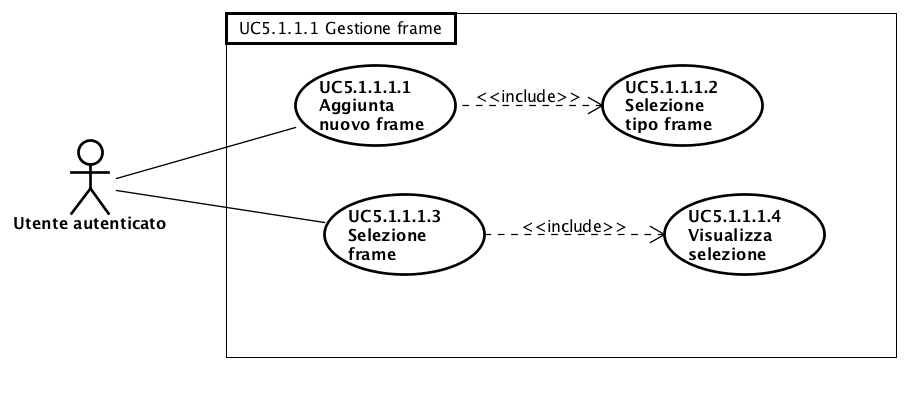
\includegraphics[scale=0.4]{diagram/UC5-1-1-1.png}
	\caption{Caso d'uso UC5.1.1.1}
	\end{center}
\end{figure}
\begin{itemize}
	\item \textbf{Precondizione:} L'utente ha scelto di modificare una presentazione;
	\item \textbf{Postcondizione:} Lo stato di qualche frame$_G$ sarà cambiato;
	\item \textbf{Descrizione:} L'utente può modificare il numero di frame$_G$, la loro gerarchia, la forma e la posizione;
	\item \textbf{Attori:} Utente autenticato;
	\item \textbf{Scenario principale:}
	\begin{enumerate}
		\item \textbf{ UC5.1.1.1.1:} \textit{ Aggiunta nuovo frame$_G$};
		\item \textbf{ UC5.1.1.1.2:} \textit{ Selezione tipo frame$_G$ };
		\item \textbf{ UC5.1.1.1.3:} \textit{ Selezione frame$_G$};
		\item \textbf{ UC5.1.1.1.4:} \textit{ Visualizza selezione}.
	\end{enumerate}
\end{itemize}
\subsection{ UC5.1.1.1.1: Aggiunta nuovo frame$_G$}

\begin{itemize}
	\item \textbf{Precondizione:} L'utente ha scelto di gestire i frame$_G$ della presentazione;
	\item \textbf{Postcondizione:} Viene aggiunto e visualizzato un frame$_G$, con la forma scelta dall'utente, nella presentazione;
	\item \textbf{Descrizione:} L'utente può aggiungere un nuovo frame$_G$ nella presentazione scegliendone la forma;
	\item \textbf{Attori:} Utente autenticato.
\end{itemize}
\subsection{ UC5.1.1.1.2: Selezione tipo frame$_G$ }

\begin{itemize}
	\item \textbf{Precondizione:} L'utente ha scelto di inserire un nuovo frame$_G$;
	\item \textbf{Postcondizione:} Il frame$_G$ da aggiungere avrà la forma selezionata dall'utente;
	\item \textbf{Descrizione:} L'utente può selezionare la forma del frame$_G$;
	\item \textbf{Attori:} Utente autenticato.
\end{itemize}
\subsection{ UC5.1.1.1.3: Selezione frame$_G$}

\begin{figure}[h]
	\begin{center}
	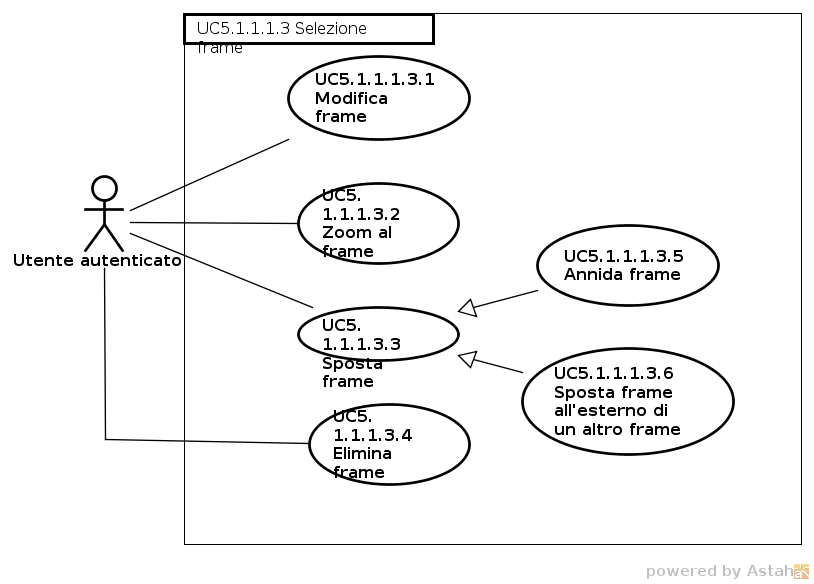
\includegraphics[scale=0.4]{diagram/UC5-1-1-1-3.png}
	\caption{Caso d'uso UC5.1.1.1.3}
	\end{center}
\end{figure}
\begin{itemize}
	\item \textbf{Precondizione:} L'utente ha scelto di gestire i frame$_G$;
	\item \textbf{Postcondizione:} Il frame$_G$ scelto dall'utente viene selezionato, l'utente ha accesso a una serie di funzionalità per quel frame$_G$;
	\item \textbf{Descrizione:} L'utente può selezionare un frame$_G$ rendendo così possibili una serie di operazioni sul frame$_G$;
	\item \textbf{Attori:} Utente autenticato;
	\item \textbf{Scenario principale:}
	\begin{enumerate}
		\item \textbf{ UC5.1.1.1.3.1:} \textit{ Modifica frame$_G$};
		\item \textbf{ UC5.1.1.1.3.2:} \textit{ Zoom al frame$_G$};
		\item \textbf{ UC5.1.1.1.3.3:} \textit{ Sposta frame$_G$};
		\item \textbf{ UC5.1.1.1.3.4:} \textit{ Elimina frame$_G$};
		\item \textbf{ UC5.1.1.1.3.5:} \textit{ Annida frame$_G$};
		\item \textbf{ UC5.1.1.1.3.6:} \textit{ Sposta frame$_G$ all'esterno di un altro frame$_G$  }.
	\end{enumerate}
\end{itemize}
\subsection{ UC5.1.1.1.3.1: Modifica frame$_G$}

\begin{itemize}
	\item \textbf{Precondizione:} Il frame$_G$ da modificare è stato selezionato;
	\item \textbf{Postcondizione:} Le modifiche apportate al frame$_G$ verranno visualizzate;
	\item \textbf{Descrizione:} L'utente può scegliere di ridimensionare un frame$_G$ già presente nella presentazione, rendendolo più piccolo o più grande o in alternativa cambiarne la forma;
	\item \textbf{Attori:} Utente autenticato.
\end{itemize}
\subsection{ UC5.1.1.1.3.2: Zoom al frame$_G$}

\begin{itemize}
	\item \textbf{Precondizione:} Il frame$_G$ è stato selezionato;
	\item \textbf{Postcondizione:} Lo zoom sarà focalizzato sul frame$_G$ scelto;
	\item \textbf{Descrizione:} L'utente può zoommare sul frame$_G$ selezionato rendendone più visibile il contenuto;
	\item \textbf{Attori:} Utente autenticato.
\end{itemize}
\subsection{ UC5.1.1.1.3.3: Sposta frame$_G$}

\begin{itemize}
	\item \textbf{Precondizione:} Il frame$_G$ è stato selezionato;
	\item \textbf{Postcondizione:} Verrà cambiata la posizione del frame$_G$;
	\item \textbf{Descrizione:} L'utente può modificare la posizione del frame$_G$;
	\item \textbf{Attori:} Utente autenticato.
\end{itemize}
\subsection{ UC5.1.1.1.3.4: Elimina frame$_G$}

\begin{itemize}
	\item \textbf{Precondizione:} Il frame$_G$ è stato selezionato;
	\item \textbf{Postcondizione:} Il frame$_G$ e gli oggetti correlati a questo vengono eliminati;
	\item \textbf{Descrizione:} L'utente può eliminare il frame$_G$;
	\item \textbf{Attori:} Utente autenticato.
\end{itemize}
\subsection{ UC5.1.1.1.3.5: Annida frame$_G$}

\begin{itemize}
	\item \textbf{Precondizione:} Il frame$_G$ è stato selezionato;
	\item \textbf{Postcondizione:} Il frame$_G$ verrà spostato all'interno di un altro frame$_G$;
	\item \textbf{Descrizione:} L'utente può trascinare un frame$_G$ all'interno di un altro frame$_G$;
	\item \textbf{Attori:} Utente autenticato.
\end{itemize}
\subsection{ UC5.1.1.1.3.6: Sposta frame$_G$ all'esterno di un altro frame$_G$}

\begin{itemize}
	\item \textbf{Precondizione:} Il frame$_G$ è stato selezionato. Il frame$_G$ si trova all'interno di un frame$_G$;
	\item \textbf{Postcondizione:} Il frame$_G$ verrà spostato all'esterno del frame$_G$ contenitore;
	\item \textbf{Descrizione:} L'utente può trascinare un frame$_G$ all'esterno del frame$_G$ che lo contiene;
	\item \textbf{Attori:} Utente autenticato.
\end{itemize}
\subsection{ UC5.1.1.1.4: Visualizza selezione}

\begin{itemize}
	\item \textbf{Precondizione:} L'utente ha selezionato un frame$_G$;
	\item \textbf{Postcondizione:} Verrà visualizzata la selezione del frame$_G$;
	\item \textbf{Descrizione:} Il frame$_G$ selezionato cambia colore;
	\item \textbf{Attori:} Utente autenticato.
\end{itemize}
\newpage
\subsection{ UC5.1.1.2: Gestione testo}

\begin{figure}[h]
	\begin{center}
	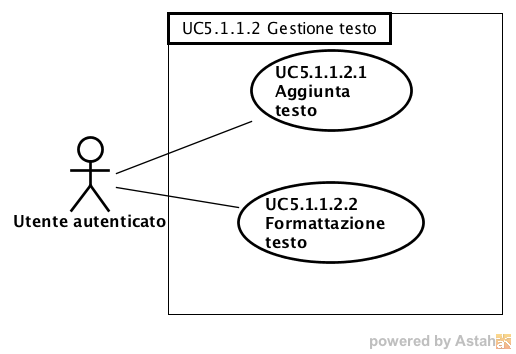
\includegraphics[scale=0.4]{diagram/UC5-1-1-2.png}
	\caption{Caso d'uso UC5.1.1.2}
	\end{center}
\end{figure}
\begin{itemize}
	\item \textbf{Precondizione:} L'utente ha scelto di modificare una presentazione;
	\item \textbf{Postcondizione:} Le operazioni sui testi verranno visualizzate;
	\item \textbf{Descrizione:} L'utente può gestire i testi della presentazione modificandoli, inserendone ed eliminandone;
	\item \textbf{Attori:} Utente autenticato;
	\item \textbf{Scenario principale:}
	\begin{enumerate}
		\item \textbf{ UC5.1.1.2.1:} \textit{ Aggiunta testo};
		\item \textbf{ UC5.1.1.2.2:} \textit{ Formattazione testo}.
	\end{enumerate}
\end{itemize}
\subsection{ UC5.1.1.2.1: Aggiunta testo}

\begin{itemize}
	\item \textbf{Precondizione:} L'utente ha scelto di gestire i testi;
	\item \textbf{Postcondizione:} Un nuovo testo sarà inserito;
	\item \textbf{Descrizione:} L'utente può inserire un nuovo testo;
	\item \textbf{Attori:} Utente autenticato.
\end{itemize}
\newpage
\subsection{ UC5.1.1.2.2: Formattazione testo}

\begin{figure}[h]
	\begin{center}
	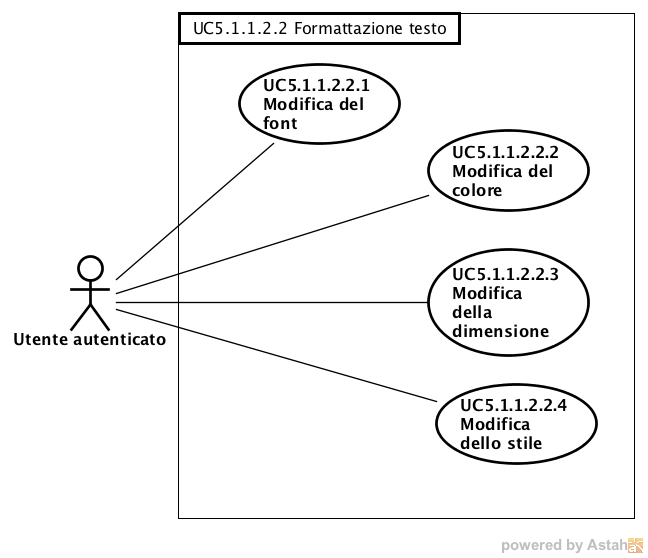
\includegraphics[scale=0.4]{diagram/UC5-1-1-2-2.png}
	\caption{Caso d'uso UC5.1.1.2.2}
	\end{center}
\end{figure}
\begin{itemize}
	\item \textbf{Precondizione:} L'utente ha scelto di gestire i testi;
	\item \textbf{Postcondizione:} La formattazione dei testi sarà modificata;
	\item \textbf{Descrizione:} L'utente può modificare la formattazione del testo scegliendo font, colore, tipologia;
	\item \textbf{Attori:} Utente autenticato;
	\item \textbf{Scenario principale:}
	\begin{enumerate}
		\item \textbf{ UC5.1.1.2.2.1:} \textit{ Modifica del font};
		\item \textbf{ UC5.1.1.2.2.2:} \textit{ Modifica del colore};
		\item \textbf{ UC5.1.1.2.2.3:} \textit{ Modifica della dimensione};
		\item \textbf{ UC5.1.1.2.2.4:} \textit{ Modifica del stile}.
	\end{enumerate}
\end{itemize}
\subsection{ UC5.1.1.2.2.1: Modifica del font}

\begin{itemize}
	\item \textbf{Precondizione:} L'utente ha scelto di modificare i testi;
	\item \textbf{Postcondizione:} I testi della presentazione avranno il font selezionato;
	\item \textbf{Descrizione:} L'utente può cambiare il font;
	\item \textbf{Attori:} Utente autenticato.
\end{itemize}
\subsection{ UC5.1.1.2.2.2: Modifica del colore}

\begin{itemize}
	\item \textbf{Precondizione:} L'utente ha scelto di modificare il colore dei testi;
	\item \textbf{Postcondizione:} Il colore dei testi verrà cambiato;
	\item \textbf{Descrizione:} L'utente può modificare il colore dei testi;
	\item \textbf{Attori:} Utente autenticato.
\end{itemize}
\subsection{ UC5.1.1.2.2.3: Modifica della dimensione }

\begin{itemize}
	\item \textbf{Precondizione:} L'utente ha scelto di modificare la dimensione dei testi;
	\item \textbf{Postcondizione:} La modifica della dimensione viene visualizzata;
	\item \textbf{Descrizione:} L'utente può modificare la dimensione;
	\item \textbf{Attori:} Utente autenticato.
\end{itemize}
\subsection{ UC5.1.1.2.2.4: Modifica del stile}

\begin{itemize}
	\item \textbf{Precondizione:} L'utente ha scelto di modificare lo stile del testo;
	\item \textbf{Postcondizione:} La modifica dello stile viene visualizzata;
	\item \textbf{Descrizione:} L'utente può scegliere un qualche stile per il testo, ad esempio: bold, italico, etc;
	\item \textbf{Attori:} Utente autenticato.
\end{itemize}
\newpage
\subsection{ UC5.1.1.3: Gestione oggetti grafici}

\begin{figure}[h]
	\begin{center}
	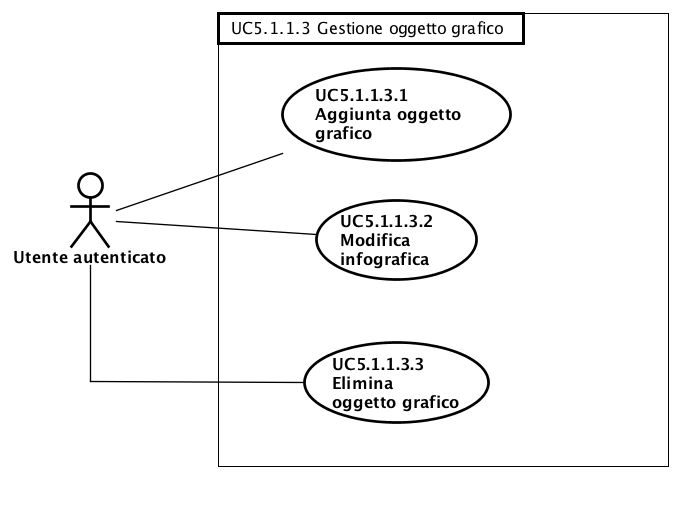
\includegraphics[scale=0.4]{diagram/UC5-1-1-3.png}
	\caption{Caso d'uso UC5.1.1.3}
	\end{center}
\end{figure}
\begin{itemize}
	\item \textbf{Precondizione:} L'utente ha scelto di modificare la presentazione;
	\item \textbf{Postcondizione:} Le modifiche apportate agli oggetti grafici scelti vengono visualizzate;
	\item \textbf{Descrizione:} L'utente può gestire tutti gli oggetti grafici messi a sua disposizione dal sistema;
	\item \textbf{Attori:} Utente autenticato;
	\item \textbf{Scenario principale:}
	\begin{enumerate}
		\item \textbf{ UC5.1.1.3.1:} \textit{ Aggiunta oggetto grafico};
		\item \textbf{ UC5.1.1.3.2:} \textit{ Modifica infografica};
		\item \textbf{ UC5.1.1.3.3:} \textit{ Elimina oggetto grafico}.
	\end{enumerate}
\end{itemize}

\newpage
\subsection{ UC5.1.1.3.1: Aggiunta oggetto grafico}

\begin{figure}[h]
	\begin{center}
	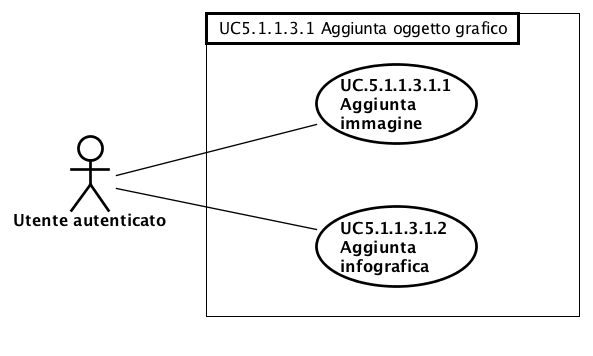
\includegraphics[scale=0.4]{diagram/UC5-1-1-3-1.png}
	\caption{Caso d'uso UC5.1.1.3.1}
	\end{center}
\end{figure}
\begin{itemize}
	\item \textbf{Precondizione:} L'utente ha scelto di aggiungere un oggetto grafico nella presentazione corrente;
	\item \textbf{Postcondizione:} L'oggetto grafico viene aggiunto e visualizzato nella presentazione corrente;
	\item \textbf{Descrizione:} L'utente può aggiungere un oggetto grafico alla presentazione;
	\item \textbf{Attori:} Utente autenticato;
	\item \textbf{Scenario principale:}
	\begin{enumerate}
		\item \textbf{ UC5.1.1.3.1.1:} \textit{ Aggiunta immagine};
		\item \textbf{ UC5.1.1.3.1.2:} \textit{ Aggiunta infografica}.
	\end{enumerate}
\end{itemize}

\newpage
\subsection{ UC5.1.1.3.1.1: Aggiunta immagine}

\begin{itemize}
	\item \textbf{Precondizione:} L'utente ha scelto di aggiungere un immagine nella presentazione corrente;
	\item \textbf{Postcondizione:} L'immagine è stata aggiunta e visualizzata nella presentazione corrente. L'immagine sarà associata ad un frame$_G$;
	\item \textbf{Descrizione:} L'utente può aggiungere un immagine alla presentazione;
	\item \textbf{Attori:} Utente autenticato.
\end{itemize}
\subsection{ UC5.1.1.3.1.2: Aggiunta infografica}

\begin{figure}[h]
	\begin{center}
	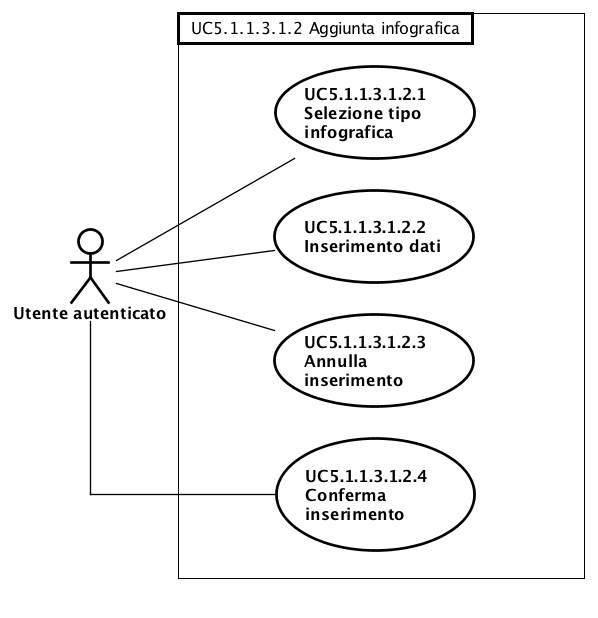
\includegraphics[scale=0.4]{diagram/UC5-1-1-3-1-2.png}
	\caption{Caso d'uso UC5.1.1.3.1.2}
	\end{center}
\end{figure}
\begin{itemize}
	\item \textbf{Precondizione:} L'utente ha scelto di aggiungere un'infografica  nella presentazione corrente;
	\item \textbf{Postcondizione:} L'infografica è stata aggiunta e visualizzata nella presentazione corrente;
	\item \textbf{Descrizione:} L'utente ha scelto di aggiungere un'infografica nella presentazione corrente, appena verrà aggiunta verrà visualizzata nella presentazione;
	\item \textbf{Attori:} Utente autenticato;
	\item \textbf{Scenario principale:}
	\begin{enumerate}
		\item \textbf{ UC5.1.1.3.1.2.1:} \textit{ Selezione tipo infografica};
		\item \textbf{ UC5.1.1.3.1.2.2:} \textit{ Inserimento dati};
		\item \textbf{ UC5.1.1.3.1.2.3:} \textit{ Annulla inserimento};
		\item \textbf{ UC5.1.1.3.1.2.4:} \textit{ Conferma inserimento}.
	\end{enumerate}
\end{itemize}
\subsection{ UC5.1.1.3.1.2.1: Selezione tipo infografica}

\begin{itemize}
	\item \textbf{Precondizione:} L'utente ha scelto di aggiungere un'infografica nella presentazione corrente;
	\item \textbf{Postcondizione:} L'utente ha selezionato un tipo di infografica. Viene visualizzata una selezione in corrispondenza dell'infografica scelta;
	\item \textbf{Descrizione:} L'utente ha scelto di aggiungere un'infogarfica nella presentazione corrente. Quindi, dovrà selezionarne un tipo. Successivamente, verrà inserita l'infografica corrispondente;
	\item \textbf{Attori:} Utente autenticato.
\end{itemize}
\subsection{ UC5.1.1.3.1.2.2: Inserimento dati}

\begin{itemize}
	\item \textbf{Precondizione:} L'utente ha scelto di aggiungere un'infografica nella presentazione corrente;
	\item \textbf{Postcondizione:} L'utente ha inserito dei dati;
	\item \textbf{Descrizione:} L'utente ha scelto di aggiungere un'infogarfica nella presentazione corrente. Quindi, dovrà inserire dei dati da visualizzare nell'infografica. Successivamente, verrà inserita l'infografica corrispondente;
	\item \textbf{Attori:} Utente autenticato.
\end{itemize}
\subsection{ UC5.1.1.3.1.2.3: Annulla inserimento}

\begin{itemize}
	\item \textbf{Precondizione:} L'utente ha deciso di annullare l'inserimento dei dati;
	\item \textbf{Postcondizione:} Viene annullato l'inserimento dei dati, e non vengono applicate modifiche all'infografica;
	\item \textbf{Descrizione:} L'utente ha scelto di aggiungere un'infogarfica nella presentazione corrente. Quindi, dovrà inserire dei dati corrispondenti. Successivamente, l'utente sceglie di annullare l'inserimento, di conseguenza non verranno applicate modifiche all'infografica;
	\item \textbf{Attori:} Utente autenticato.
\end{itemize}
\subsection{ UC5.1.1.3.1.2.4: Conferma inserimento}

\begin{itemize}
	\item \textbf{Precondizione:} L'utente ha concluso l'inserimento dei dati e ha deciso di confermarli;
	\item \textbf{Postcondizione:} Viene confermato l'inserimento. Vengono visualizzate le modifiche;
	\item \textbf{Descrizione:} L'utente ha scelto di aggiungere un'infogarfica nella presentazione corrente. Quindi, dovrà inserire dei dati corrispondenti. Successivamente, l'utente sceglie di confermare l'inserimento, di conseguenza verranno applicate modifiche all'infografica e saranno visualizzate le modifiche;
	\item \textbf{Attori:} Utente autenticato.
\end{itemize}
\subsection{ UC5.1.1.3.2: Modifica infografica}

\begin{figure}[h]
	\begin{center}
	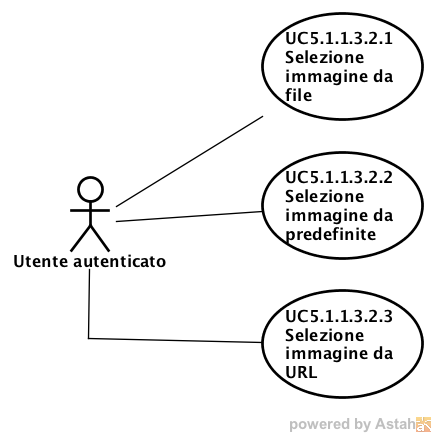
\includegraphics[scale=0.4]{diagram/UC5-1-1-3-2.png}
	\caption{Caso d'uso UC5.1.1.3.2}
	\end{center}
\end{figure}
\begin{itemize}
	\item \textbf{Precondizione:} L'utente ha scelto di modificare un'infografica per la presentazione corrente;
	\item \textbf{Postcondizione:} L'infografica è stata modificata e le modiche vengono visualizzate;
	\item \textbf{Descrizione:} L'utente ha scelto di modificare un'infografica nella presentazione corrente, appena verrà modificata, sarà visualizzata la modifica nella presentazione;
	\item \textbf{Attori:} Utente autenticato;
	\item \textbf{Scenario principale:}
	\begin{enumerate}
		\item \textbf{ UC5.1.1.3.2.1:} \textit{ Modifica tipologia};
		\item \textbf{ UC5.1.1.3.2.2:} \textit{ Modifica dati};
		\item \textbf{ UC5.1.1.3.2.3:} \textit{ Conferma modifiche};
		\item \textbf{ UC5.1.1.3.2.4:} \textit{ Annulla modifiche}.
	\end{enumerate}
\end{itemize}
\subsection{ UC5.1.1.3.2.1: Modifica tipologia}

\begin{itemize}
	\item \textbf{Precondizione:} L'utente ha scelto un infografica e ne vuole modificare il tipo;
	\item \textbf{Postcondizione:} Il tipo di infografica viene modificato e vengono visualizzate le modifiche;
	\item \textbf{Descrizione:} L'utente ha scelto di modificare la tipologia di un'infografica nella presentazione corrente, appena verrà modificata, sarà visualizzata la modifica nella presentazione;
	\item \textbf{Attori:} Utente autenticato.
\end{itemize}
\subsection{ UC5.1.1.3.2.2: Modifica dati}

\begin{itemize}
	\item \textbf{Precondizione:} L'utente ha scelto di modificare i dati per l'infografica;
	\item \textbf{Postcondizione:} I dati sono modificati. Vengono visualizzate le modifiche;
	\item \textbf{Descrizione:} L'utente può modificare i dati relativi ad un'infografica;
	\item \textbf{Attori:} Utente autenticato.
\end{itemize}
\subsection{ UC5.1.1.3.2.3: Conferma modifiche}

\begin{itemize}
	\item \textbf{Precondizione:} L'utente ha scelto di confermare le modifiche per l'infografica;
	\item \textbf{Postcondizione:} Sono state confermate e visualizzate le modifiche;
	\item \textbf{Descrizione:} L'utente ha scelto di confermare le modifiche di un'infografica nella presentazione corrente, appena verrà confermata la modifica sarà visualizzata la modifica nella presentazione;
	\item \textbf{Attori:} Utente autenticato.
\end{itemize}
\subsection{ UC5.1.1.3.2.4: Annulla modifiche}

\begin{itemize}
	\item \textbf{Precondizione:} L'utente ha scelto di annullare le modifiche per l'infografica;
	\item \textbf{Postcondizione:} Sono state annullate le modifiche;
	\item \textbf{Descrizione:} L'utente ha scelto di annullare le modifiche di un'infogarfica nella presentazione corrente. Quindi, non verranno applicate modifiche all'infografica;
	\item \textbf{Attori:} Utente autenticato.
\end{itemize}
\subsection{ UC5.1.1.3.3: Elimina oggetto grafico}

\begin{itemize}
	\item \textbf{Precondizione:} L'utente ha scelto di eliminare un oggetto grafico;
	\item \textbf{Postcondizione:} L'oggetto grafico è stato eliminato;
	\item \textbf{Descrizione:} L'utente ha scelto di eliminare un oggetto grafico. Quindi, verrà elimitato l'oggetto grafico corrispondente;
	\item \textbf{Attori:} Utente autenticato.
\end{itemize}
\subsection{ UC5.1.1.4: Modifica tema}

\begin{figure}[h]
	\begin{center}
	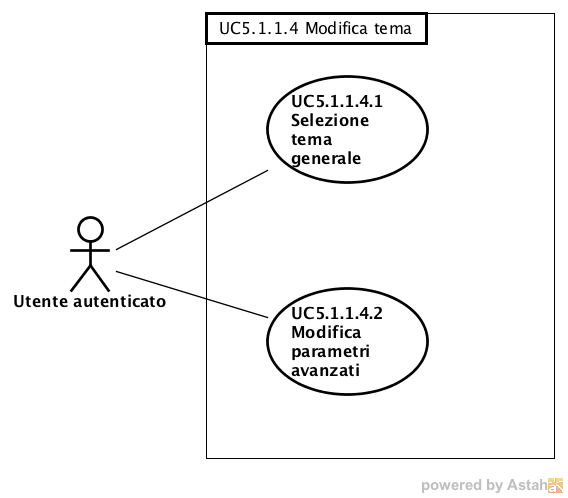
\includegraphics[scale=0.4]{diagram/UC5-1-1-4.png}
	\caption{Caso d'uso UC5.1.1.4}
	\end{center}
\end{figure}
\begin{itemize}
	\item \textbf{Precondizione:} L’utente ha scelto di modificare il tema per la presentazione corrente;
	\item \textbf{Postcondizione:} Il tema è stato modificato e le modifiche vengono visualizzate;
	\item \textbf{Descrizione:} L'utente ha scelto di modificare il tema della presentazione corrente, appena verrà modificato, sarà visualizzata la modifica nella presentazione;
	\item \textbf{Attori:} Utente autenticato;
	\item \textbf{Scenario principale:}
	\begin{enumerate}
		\item \textbf{ UC5.1.1.4.1:} \textit{ Selezione tema generale};
		\item \textbf{ UC5.1.1.4.2:} \textit{ Modifica parametri avanzati}.
	\end{enumerate}
\end{itemize}
\subsection{ UC5.1.1.4.1: Selezione tema generale}

\begin{itemize}
	\item \textbf{Precondizione:} L'utente ha scelto di selezionare un tema generale;
	\item \textbf{Postcondizione:} Il tema è stato applicato e viene visualizzato;
	\item \textbf{Descrizione:} L'utente ha scelto di selezionare un tema generale. Successivamente, sarà applicato e visualizzato;
	\item \textbf{Attori:} Utente autenticato.
\end{itemize}
\subsection{ UC5.1.1.4.2: Modifica parametri avanzati}

\begin{figure}[h]
	\begin{center}
	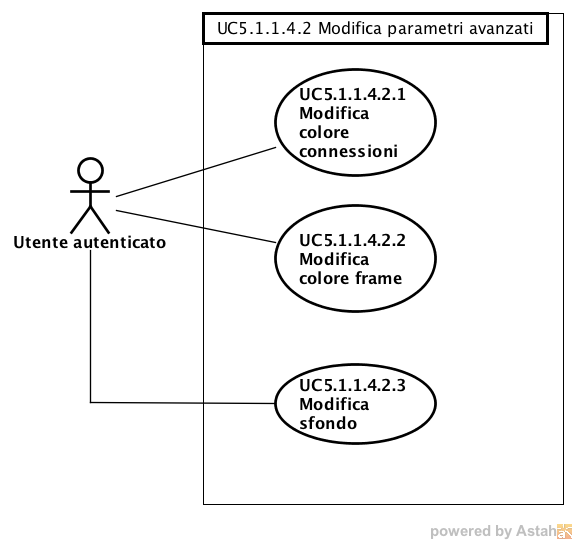
\includegraphics[scale=0.4]{diagram/UC5-1-1-4-2.png}
	\caption{Caso d'uso UC5.1.1.4.2}
	\end{center}
\end{figure}
\begin{itemize}
	\item \textbf{Precondizione:} L'utente ha scelto di modificare i parametri avanzati;
	\item \textbf{Postcondizione:} I parametri avanzati sono modificati e si visualizzano le modifiche;
	\item \textbf{Descrizione:} L'utente decide di modificare i parametri avanzati, successivamente verranno visualizzate le modifiche;
	\item \textbf{Attori:} Utente autenticato;
	\item \textbf{Scenario principale:}
	\begin{enumerate}
		\item \textbf{ UC5.1.1.4.2.1:} \textit{ Modifica colore connessioni};
		\item \textbf{ UC5.1.1.4.2.2:} \textit{ Modifica colore frame$_G$};
		\item \textbf{ UC5.1.1.4.2.3:} \textit{ Modifica sfondo}.
	\end{enumerate}
\end{itemize}
\subsection{ UC5.1.1.4.2.1: Modifica colore connessioni}

\begin{itemize}
	\item \textbf{Precondizione:} L'utente ha scelto di modificare il colore delle connessioni;
	\item \textbf{Postcondizione:} Il colore delle connessioni è stato modificato e vengono visualizzate le modifiche;
	\item \textbf{Descrizione:} L'utente ha scelto di modificare il colore delle connessioni.  Successivamente, dopo la scelta del colore, verrà modificato il colore e visualizzata la modifica;
	\item \textbf{Attori:} Utente autenticato.
\end{itemize}
\subsection{ UC5.1.1.4.2.2: Modifica colore frame$_G$}

\begin{itemize}
	\item \textbf{Precondizione:} L'utente ha scelto di modificare il colore del frame$_G$;
	\item \textbf{Postcondizione:} Il colore del frame$_G$ è stato modificato e vengono visualizzate le modifiche;
	\item \textbf{Descrizione:} L'utente ha scelto di modificare il colore del frame$_G$.  Successivamente, dopo la scelta del colore, verrà modificato il colore e visualizzata la modifica;
	\item \textbf{Attori:} Utente autenticato.
\end{itemize}
\subsection{ UC5.1.1.4.2.3: Modifica sfondo}

\begin{figure}[h]
	\begin{center}
	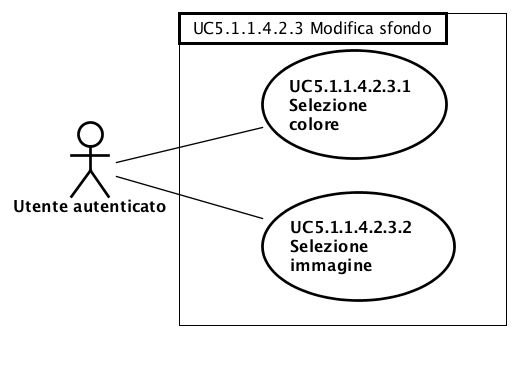
\includegraphics[scale=0.4]{diagram/UC5-1-1-4-2-3.png}
	\caption{Caso d'uso UC5.1.1.4.2.3}
	\end{center}
\end{figure}
\begin{itemize}
	\item \textbf{Precondizione:} L'utente ha scelto di modificare lo sfondo;
	\item \textbf{Postcondizione:} Lo sfondo viene modificato e viene visualizzata la modifica;
	\item \textbf{Descrizione:} L'utente ha scelto di modificare lo sfondo.  Successivamente, verrà modificato e visualizzata la modifica;
	\item \textbf{Attori:} Utente autenticato;
	\item \textbf{Scenario principale:}
	\begin{enumerate}
		\item \textbf{ UC5.1.1.4.2.3.1:} \textit{ Selezione colore};
		\item \textbf{ UC5.1.1.4.2.3.2:} \textit{ Selezione immagine}.
	\end{enumerate}
\end{itemize}
\subsection{ UC5.1.1.4.2.3.1: Selezione colore}

\begin{itemize}
	\item \textbf{Precondizione:} L'utente ha scelto di modificare il colore per lo sfondo;
	\item \textbf{Postcondizione:} Il colore di sfondo è stato selezionato e viene visualizzata la selezione;
	\item \textbf{Descrizione:} L'utente dovrà selezionare un colore.  Successivamente, viene visualizzata la selezione;
	\item \textbf{Attori:} Utente autenticato.
\end{itemize}
\subsection{ UC5.1.1.4.2.3.2: Selezione immagine}

\begin{figure}[h]
	\begin{center}
	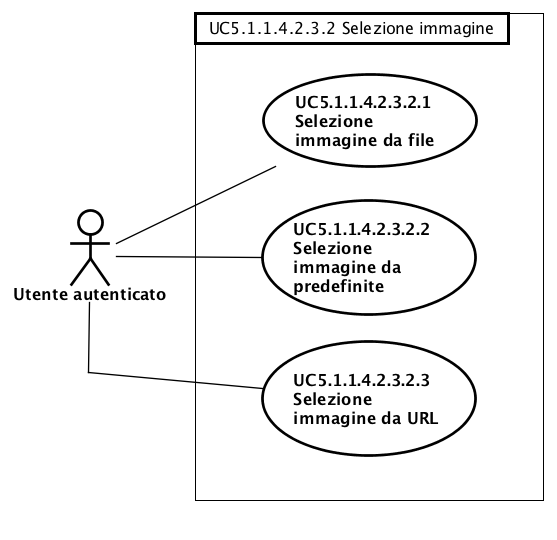
\includegraphics[scale=0.4]{diagram/UC5-1-1-4-2-3-2.png}
	\caption{Caso d'uso UC5.1.1.4.2.3.2}
	\end{center}
\end{figure}
\begin{itemize}
	\item \textbf{Precondizione:} L'utente ha scelto di selezionare un'immagine di sfondo;
	\item \textbf{Postcondizione:} L'immagine di sfondo è stata selezionata e viene visualizzata la selezione;
	\item \textbf{Descrizione:} L'utente ha scelto di selezionare un'immagine di sfondo. Successivamente, verrà visualizzata la selezione;
	\item \textbf{Attori:} Utente autenticato;
	\item \textbf{Scenario principale:}
	\begin{enumerate}
		\item \textbf{ UC5.1.1.4.2.3.2.1:} \textit{ Selezione immagine da file};
		\item \textbf{ UC5.1.1.4.2.3.2.2:} \textit{ Selezione immagine da predefinite};
		\item \textbf{ UC5.1.1.4.2.3.2.3:} \textit{ Selezione immagine da URL$_G$}.
	\end{enumerate}
\end{itemize}
\subsection{ UC5.1.1.4.2.3.2.1: Selezione immagine da file}

\begin{itemize}
	\item \textbf{Precondizione:} l’utente ha scelto di selezionare l’immagine da file;
	\item \textbf{Postcondizione:} l’immagine selezionata viene applicata allo sfondo della presentazione;
	\item \textbf{Descrizione:} l’utente sceglie l’immagine dal proprio dispositivo tramite una finestra apposita;
	\item \textbf{Attori:} Utente autenticato.
\end{itemize}
\subsection{ UC5.1.1.4.2.3.2.2: Selezione immagine da predefinite}

\begin{itemize}
	\item \textbf{Precondizione:} l’utente ha scelto di selezionare l’immagine tra quelle fornite dal sistema;
	\item \textbf{Postcondizione:} l’immagine selezionata viene applicata allo sfondo della presentazione;
	\item \textbf{Descrizione:} vengono mostrate una serie di immagini fornite dal sistema dalle quali l’utente può scegliere quella da impostare come sfondo;
	\item \textbf{Attori:} Utente autenticato.
\end{itemize}
\subsection{ UC5.1.1.4.2.3.2.3: Selezione immagine da URL$_G$}

\begin{itemize}
	\item \textbf{Precondizione:} l’utente ha scelto di selezionare l’immagine fornendo il relativo URL$_G$;
	\item \textbf{Postcondizione:} l’immagine selezionata viene applicata allo sfondo della presentazione;
	\item \textbf{Descrizione:} viene chiesto di inserire l’URL$_G$ corrispondente all’immagine;
	\item \textbf{Attori:} Utente autenticato.
\end{itemize}

\newpage
\subsection{ UC5.1.1.5: Gestione cammino}

\begin{figure}[h]
	\begin{center}
	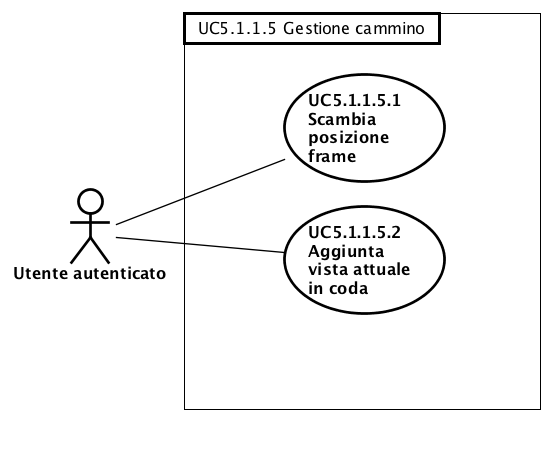
\includegraphics[scale=0.4]{diagram/UC5-1-1-5.png}
	\caption{Caso d'uso UC5.1.1.5}
	\end{center}
\end{figure}
\begin{itemize}
	\item \textbf{Precondizione:} L’utente si trova nell’editor e decide di gestire il cammino presentativo della presentazione;
	\item \textbf{Postcondizione:} L’utente ha terminato la gestione del cammino presentativo e visualizza eventuali cambiamenti;
	\item \textbf{Descrizione:} L’utente si presta a gestire il cammino presentativo, cioè l’ordine in cui vengono visualizzati i vari frame$_G$;
	\item \textbf{Attori:} Utente autenticato;
	\item \textbf{Scenario principale:}
	\begin{enumerate}
		\item \textbf{ UC5.1.1.5.1:} \textit{ Scambia posizione frame$_G$};
		\item \textbf{ UC5.1.1.5.2:} \textit{ Aggiunta vista attuale in coda}.
	\end{enumerate}
\end{itemize}
\subsection{ UC5.1.1.5.1: Scambia posizione frame$_G$}

\begin{itemize}
	\item \textbf{Precondizione:} L’utente si trova nell’editor e ha deciso di gestire il cammino presentativo scambiando la posizione dei frame$_G$;
	\item \textbf{Postcondizione:} I frame$_G$ sono stati scambiati correttamente e il nuovo cammino viene visualizzato a video;
	\item \textbf{Descrizione:} L’utente può scambiare di posizione i vari frame$_G$ semplicemente utilizzando la funzione di drag and drop$_G$, oppure assegnando un numero al frame$_G$, che corrisponde alla posizione in cui il frame$_G$ verrà visualizzato;
	\item \textbf{Attori:} Utente autenticato.
\end{itemize}
\subsection{ UC5.1.1.5.2: Aggiunta vista attuale in coda}

\begin{itemize}
	\item \textbf{Precondizione:} L’utente si trova nell’editor e ha deciso di gestire il cammino presentativo aggiungendo in coda la vista attuale;
	\item \textbf{Postcondizione:} La vista attuale viene aggiunta in coda al cammino presentativo che quindi avrà un passo in più;
	\item \textbf{Descrizione:} L’utente, durante la gestione del cammino presentativo, può scegliere di aggiungere in coda la vista attuale, ovvero la vista della presentazione al livello di zoom presente al momento dell’aggiunta;
	\item \textbf{Attori:} Utente autenticato.
\end{itemize}
\subsection{ UC5.1.1.6: Avvia anteprima}

\begin{itemize}
	\item \textbf{Precondizione:} L’utente si trova all’interno dell’editor e decide di avviare l’anteprima della presentazione con le eventuali modifiche effettuate;
	\item \textbf{Postcondizione:} La presentazione viene avviata correttamente a schermo intero con tutte le eventuali modifiche effettuate da parte dell’utente;
	\item \textbf{Descrizione:} In qualsiasi momento durante la modifica della presentazione l’utente può scegliere di avviare l’anteprima della presentazione. Ciò comporta l’avvio della presentazione stessa in modalità a schermo intero con tutte le eventuali modifiche apportate fino a quel momento da parte dell’utente;
	\item \textbf{Attori:} Utente autenticato.
\end{itemize}
\subsection{ UC5.1.1.7: Salvataggio}

\begin{itemize}
	\item \textbf{Precondizione:} L’utente si trova all’interno dell’editor e decide di salvare la presentazione;
	\item \textbf{Postcondizione:} La presentazione è stata correttamente salvata con tutte le eventuali modifiche apportate dall’utente;
	\item \textbf{Descrizione:} In qualsiasi momento durante la modifica della presentazione l’utente può decidere di salvare le modifiche fatte fino a quel momento. Il sistema implementerà anche una funzione di salvataggio automatico;
	\item \textbf{Attori:} Utente autenticato.
\end{itemize}
\subsection{ UC5.1.1.8: Annulla la modifica}

\begin{itemize}
	\item \textbf{Precondizione:} L’utente si trova nell’editor ed ha effettuato una modifica alla presentazione;
	\item \textbf{Postcondizione:} La modifica poco prima effettuata è stata annullata;
	\item \textbf{Descrizione:} In qualsiasi istante durante la modifica della presentazione l’utente, dopo una modifica, può decidere di annullare l’ultima effettuata;
	\item \textbf{Attori:} Utente autenticato.
\end{itemize}
\subsection{ UC5.1.1.9: Ripristina la modifica annullata}

\begin{itemize}
	\item \textbf{Precondizione:} L’utente ha appena annullato una modifica;
	\item \textbf{Postcondizione:} La modifica precedentemente annullata è stata ripristinata correttamente;
	\item \textbf{Descrizione:} L’utente in qualsiasi momento, dopo aver annullato una modifica, può scegliere di ripristinarla;
	\item \textbf{Attori:} Utente autenticato.
\end{itemize}
\subsection{ UC5.1.2: Eliminazione presentazione}

\begin{itemize}
	\item \textbf{Precondizione:} L'utente ha selezionato una presentazione;
	\item \textbf{Postcondizione:} La presentazione verrà eliminata;
	\item \textbf{Descrizione:} L'utente può eliminare una presentazione;
	\item \textbf{Attori:} Utente autenticato.
\end{itemize}
\subsection{ UC5.1.3: Conferma eliminazione }

\begin{itemize}
	\item \textbf{Precondizione:} L'utente ha scelto di eliminare una presentazione;
	\item \textbf{Postcondizione:} L'utente conferma l'eliminazione concludendo il processo;
	\item \textbf{Descrizione:} L'utente deve confermare la propria intenzione di eliminare una presentazione;
	\item \textbf{Attori:} Utente autenticato.
\end{itemize}
\subsection{ UC5.1.4: Condivisione presentazione }

\begin{itemize}
	\item \textbf{Precondizione:} L'utente ha selezionato una presentazione;
	\item \textbf{Postcondizione:} La presentazione corrente sarà resa accessibile a qualunque utente tramite un URL;
	\item \textbf{Descrizione:} L'utente può condividere una propria presentazione rendendola accessibile, in lettura, anche a utenti esterni;
	\item \textbf{Attori:} Utente autenticato.
\end{itemize}
\subsection{ UC5.1.5: Esportazione poster}

\begin{itemize}
	\item \textbf{Precondizione:} L'utente ha selezionato una presentazione;
	\item \textbf{Postcondizione:} Viene generata un'immagine contenente l'intera presentazione;
	\item \textbf{Descrizione:} L'utente può decidere di esportare, in un formato che sceglierà, l'immagine della presentazione scelta;
	\item \textbf{Attori:} Utente autenticato.
\end{itemize}
\subsection{ UC5.1.6: Download presentazione$_G$}

\begin{itemize}
	\item \textbf{Precondizione:} L'utente ha scelto di esportare una presentazione;
	\item \textbf{Postcondizione:} La presentazione esportata in un formato scelto verrà scaricata;
	\item \textbf{Descrizione:} L'utente, scegliendo di esportare la presentazione selezionata, scarica il file contenente l'immagine;
	\item \textbf{Attori:} Utente autenticato.
\end{itemize}
\subsection{ UC5.1.7: Stampa presentazione }

\begin{itemize}
	\item \textbf{Precondizione:} L'utente ha selezionato una presentazione;
	\item \textbf{Postcondizione:} La richiesta di stampa verrà inviata al sistema operativo;
	\item \textbf{Descrizione:} L'utente può scegliere di stampare la propria presentazione;
	\item \textbf{Attori:} Utente autenticato.
\end{itemize}
\subsection{ UC5.1.8: Avvio sessione live}

\begin{itemize}
	\item \textbf{Precondizione:} L'utente ha selezionato una presentazione;
	\item \textbf{Postcondizione:} Viene generato un URL alla presentazione avviata, che gli utenti esterni potranno usare per assistere alla presentazione;
	\item \textbf{Descrizione:} L'utente può avviare una presentazione remota e tutti gli utenti in possesso dell' URL generato potranno assistere visualizzando in tempo reale il susseguirsi delle slide;
	\item \textbf{Attori:} Utente autenticato.
\end{itemize}

\newpage
\subsection{ UC5.1.9: Avvio presentazione }

\begin{figure}[h]
	\begin{center}
	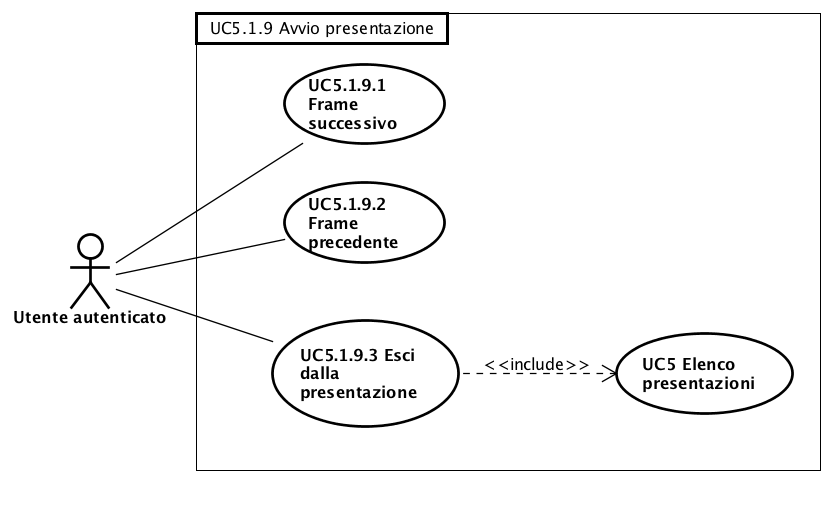
\includegraphics[scale=0.4]{diagram/UC5-1-9.png}
	\caption{Caso d'uso UC5.1.9}
	\end{center}
\end{figure}
\begin{itemize}
	\item \textbf{Precondizione:} L'utente ha selezionato una presentazione;
	\item \textbf{Postcondizione:} Viene visualizzata la presentazione con la relativa interfaccia;
	\item \textbf{Descrizione:} L'utente può avviare una presentazione e gestire il susseguirsi delle slides andando avanti o indietro nel percorso di questa;
	\item \textbf{Attori:} Utente autenticato;
	\item \textbf{Scenario principale:}
	\begin{enumerate}
		\item \textbf{ UC5.1.9.1:} \textit{ Frame$_G$ successivo};
		\item \textbf{ UC5.1.9.2:} \textit{ Frame$_G$ precedente};
		\item \textbf{ UC5.1.9.3:} \textit{ Esci dalla presentazione }.
	\end{enumerate}
\end{itemize}
\subsection{ UC5.1.9.1: Frame$_G$ successivo}

\begin{itemize}
	\item \textbf{Precondizione:} L'utente ha avviato una presentazione;
	\item \textbf{Postcondizione:} Viene visualizzato il frame$_G$ successivo, su cui viene fatto lo zoom;
	\item \textbf{Descrizione:} L'utente può avanzare nella presentazione visualizzando il frame$_G$ successivo;
	\item \textbf{Attori:} Utente autenticato.
\end{itemize}
\subsection{ UC5.1.9.2: Frame$_G$ precedente}

\begin{itemize}
	\item \textbf{Precondizione:} L'utente ha avviato una presentazione e ha eseguito almeno un avanzamento nel percorso dei frame$_G$;
	\item \textbf{Postcondizione:} Il frame$_G$ precedente viene visualizzato facendone lo zoom;
	\item \textbf{Descrizione:} L'utente può retrocedere nella visualizzazione della presentazione;
	\item \textbf{Attori:} Utente autenticato.
\end{itemize}
\subsection{ UC5.1.9.3: Esci dalla presentazione }

\begin{itemize}
	\item \textbf{Precondizione:} Una presentazione è stata avviata;
	\item \textbf{Postcondizione:} L'utente torna alla schermata con l'elenco delle presentazioni;
	\item \textbf{Descrizione:} L'utente può scegliere di terminare la presentazione;
	\item \textbf{Attori:} Utente autenticato.
\end{itemize}
\subsection{ UC5.2: Visualizzazione anteprima }

\begin{itemize}
	\item \textbf{Precondizione:} L'utente ha selezionato una presentazione;
	\item \textbf{Postcondizione:} Viene visualizzata l'anteprima della presentazione selezionata;
	\item \textbf{Descrizione:} L'utente può scegliere di visualizzare l'anteprima della presentazione;
	\item \textbf{Attori:} Utente autenticato.
\end{itemize}

\newpage
\subsection{ UC6: Modifica dati account}

\begin{figure}[h]
	\begin{center}
	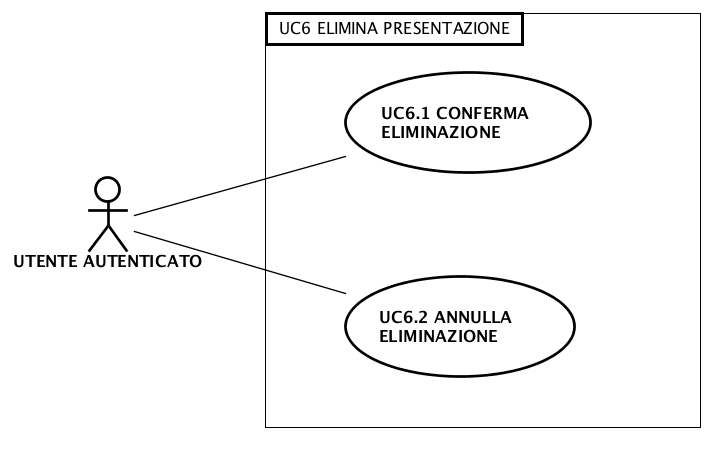
\includegraphics[scale=0.4]{diagram/UC6.png}
	\caption{Caso d'uso UC6}
	\end{center}
\end{figure}
\begin{itemize}
	\item \textbf{Precondizione:} L’utente autenticato è entrato nel sistema ed ha intenzione di modificare i propri dati dell’account;
	\item \textbf{Postcondizione:} I dati dell’utente sono stati correttamente modificati;
	\item \textbf{Descrizione:} L’utente può modificare i propri dati inseriti in fase di registrazione;
	\item \textbf{Attori:} Utente autenticato;
	\item \textbf{Scenario principale:}
	\begin{enumerate}
		\item \textbf{ UC6.1:} \textit{ Modifica password};
		\item \textbf{ UC6.2:} \textit{ Modifica e-mail};
		\item \textbf{ UC6.3:} \textit{ Conferma modifica};
		\item \textbf{ UC6.4:} \textit{ Annulla modifica}.
	\end{enumerate}
\end{itemize}

\newpage
\subsection{ UC6.1: Modifica password}

\begin{figure}[h]
	\begin{center}
	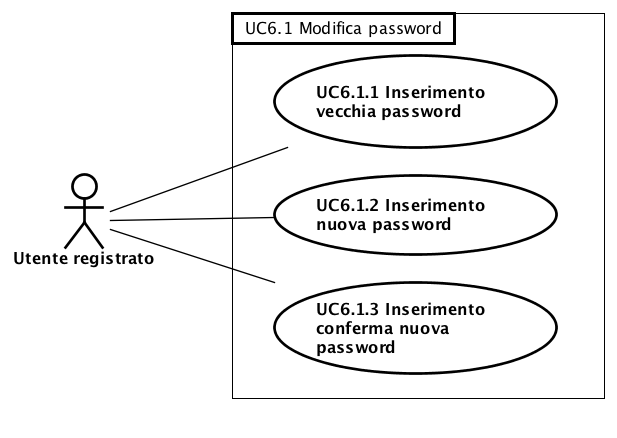
\includegraphics[scale=0.4]{diagram/UC6-1.png}
	\caption{Caso d'uso UC6.1}
	\end{center}
\end{figure}
\begin{itemize}
	\item \textbf{Precondizione:} L’utente è entrato nella sezione dedicata alla modifica dei dati dell’account ed ha deciso di modificare la password. Deve inoltre conoscere la password corrente;
	\item \textbf{Postcondizione:} La password è stata correttamente modificata;
	\item \textbf{Descrizione:} L’utente può scegliere di modificare la password una volta entrato nella sezione che permette la modifica dei propri dati;
	\item \textbf{Attori:} Utente autenticato;
	\item \textbf{Scenario principale:}
	\begin{enumerate}
		\item \textbf{ UC6.1.1:} \textit{ Inserimento vecchia password};
		\item \textbf{ UC6.1.2:} \textit{ Inserimento nuova password};
		\item \textbf{ UC6.1.3:} \textit{ Inserimento conferma nuova password}.
	\end{enumerate}
\end{itemize}
\subsection{ UC6.1.1: Inserimento vecchia password}

\begin{itemize}
	\item \textbf{Precondizione:} L’utente è entrato nella sezione dedicata alla modifica dei dati dell’account ed ha deciso di modificare la password;
	\item \textbf{Postcondizione:} L’utente ha correttamente inserito la vecchia password;
	\item \textbf{Descrizione:} L’utente inserisce la vecchia password nel campo dedicato;
	\item \textbf{Attori:} Utente autenticato.
\end{itemize}
\subsection{ UC6.1.2: Inserimento nuova password}

\begin{itemize}
	\item \textbf{Precondizione:} L’utente è entrato nella sezione dedicata alla modifica dei dati dell’account ed ha deciso di modificare la password;
	\item \textbf{Postcondizione:}  L’utente ha correttamente inserito la nuova password;
	\item \textbf{Descrizione:} L’utente inserisce la nuova password nel campo dedicato;
	\item \textbf{Attori:} Utente autenticato.
\end{itemize}
\subsection{ UC6.1.3: Inserimento conferma nuova password}

\begin{itemize}
	\item \textbf{Precondizione:} L’utente è entrato nella sezione dedicata alla modifica dei dati dell’account ed ha deciso di modificare la password;
	\item \textbf{Postcondizione:} L’utente ha correttamente inserito la conferma della nuova password;
	\item \textbf{Descrizione:} L’utente inserisce la conferma della nuova password nel campo dedicato e deve corrispondere a quella inserita nel caso d’uso UC6.1.2;
	\item \textbf{Attori:} Utente autenticato.
\end{itemize}
\subsection{ UC6.2: Modifica e-mail}

\begin{itemize}
	\item \textbf{Precondizione:} L’utente è entrato nella sezione dedicata alla modifica dei dati dell’account ed ha deciso di modificare l’indirizzo e-mail;
	\item \textbf{Postcondizione:} L’utente ha correttamente modificato il proprio indirizzo e-mail;
	\item \textbf{Descrizione:} L’utente inserisce il nuovo indirizzo e-mail al posto di quello precedente;
	\item \textbf{Attori:} Utente autenticato.
\end{itemize}
\subsection{ UC6.3: Conferma modifica}

\begin{itemize}
	\item \textbf{Precondizione:} L’utente è entrato nella sezione dedicata alla modifica dei dati dell’account e ha correttamente compilato i campi che desidera modificare;
	\item \textbf{Postcondizione:} Vengono correttamente modificati i dati e visualizzato un messaggio che conferma l’avvenuta modifica;
	\item \textbf{Descrizione:} L’utente conferma che desidera modificare i dati del proprio account con quelli appena inseriti;
	\item \textbf{Attori:} Utente autenticato.
\end{itemize}
\subsection{ UC6.4: Annulla modifica}

\begin{itemize}
	\item \textbf{Precondizione:} L’utente è entrato nella sezione dedicata alla modifica dei dati dell’account;
	\item \textbf{Postcondizione:} L’utente interrompe la modifica dei dati del proprio account che quindi non vengono modificati;
	\item \textbf{Descrizione:} L’utente interrompe la modifica dei dati dell’account lasciando la pagina dedicata prima di confermare la modifica;
	\item \textbf{Attori:} Utente autenticato.
\end{itemize}
\subsection{ UC7: Nuova presentazione}

\begin{itemize}
	\item \textbf{Precondizione:} L’utente si trova all’interno del sistema;
	\item \textbf{Postcondizione:} Viene creata una nuova presentazione e aperto l’editor per la modifica, dopo aver chiesto all’utente di selezionare un template$_G$ di partenza;
	\item \textbf{Descrizione:} L’utente che decide di creare una nuova presentazione deve per prima cosa selezionare un template$_G$ dal quale partire, che all’occorrenza può essere anche vuoto. In seguito viene aperto l’editor con il template$_G$ selezionato e si procede analogamente alla modifica di una presentazione già esistente;
	\item \textbf{Attori:} Utente autenticato.
\end{itemize}
\subsection{ UC8: Selezione template$_G$}

\begin{itemize}
	\item \textbf{Precondizione:} L’utente ha scelto di creare una nuova presentazione;
	\item \textbf{Postcondizione:} Viene selezionato il template$_G$ come base di partenza per la nuova presentazione e aperto l’editor;
	\item \textbf{Descrizione:} L’utente sceglie un template$_G$ tra quelli resi disponibili dal sistema, tra i quali quello vuoto;
	\item \textbf{Attori:} Utente autenticato.
\end{itemize}
\subsection{ UC9: Visualizza presentazione condivisa}

\begin{itemize}
	\item \textbf{Precondizione:} L’utente vuole avviare una presentazione. È necessario che l’utente disponga dell'URL corrispondente a tale presentazione;
	\item \textbf{Postcondizione:} L’utente ha correttamente inserito l'URL nel browser$_G$ e la presentazione è stata avviata;
	\item \textbf{Descrizione:} L’utente, in possesso dell'URL per la condivisione di una presentazione, lo inserisce nella barra degli indirizzi del browser$_G$ e automaticamente il sistema avvia la presentazione corrispondente all'URL inserito;
	\item \textbf{Attori:} Utente.
\end{itemize}